\chapter{Mètrica i anàlisi}

Al tractar-se d’un conjunt de mostres balancejat, les mètriques es simplifiquen bastant. Per exemple, el valor que s’obté d’accuracy és fiable. En unes dades no balancejades, el valor podria ser molt alt però les prediccions dolentes, i per tant s’hauria d’utilitzar F1-Score. El model que s’està creant només es vol per saber si un tweet és positiu o negatiu, sense donar més importància a un o l’alte. L’accuracy ens permet saber exactament això, el percentatge de prediccions ben fetes.

Si per altra banda es volgués filtrar els tweets tal que només es mostrin els que són positius, s’hauria d’utilitzar una altra mètrica. La precission ens seria una bona mètrica, doncs calcula el percentatge de prediccions positives correctes d’entre el total de  prediccions positives. Un precission alt permetria assegurar-nos que tots els tweets que passen el filtre són positius.

D’altre banda, si l’objectiu sigués permetre tants positius com sigui possible, sense importar els negatius que es colessin, s’hauria de mirar el Recall.

De totes formes, per aquesta pràctica ambdues classes són igual d’importants i es mirarà l’accuracy.\\

Les proves efectuades a la pràctica s’han realitzat amb un  “K-Fold Cross Validation” de 10 folds. Per aconseguir la mètrica simplement es fa una mitjana de les 10 mètriques obtingudes. Al haver-hi més d’una predicció, no és suficient sabent la mitjana. Cal comprovar també que els resultats siguin consistents. Ajudant-se de la desviació estàndard de totes les mètriques es pot estar segur que són consistents.

Els resultats obtinguts són una Accuracy de 75\% amb desviació estàndard de 0.001. Si bé no són excepcionalment bons, almenys les prediccions són consistents entre elles.

La matriu de confusió inferior mostra com estan distribuïdes les classificacions. Sumant els TP i TN \(45 + 30 = 75\) es pot veure que dona l’accuracy prèviament mencionada. 
També es pot veure que és bastant més capaç de classificar correctament els tweets negatius que els positius. \\

Per últim, utilitzar el “Leave One Out” no és plausible ja que es té moltes mostres i el temps d’execució triga molt. \\

La figura ~\ref{fig:matriuConfusio} mostra els resultats esmentats anteriorment \footnote{Cal anotar que  la matriu està normalitzada tant per files com per columnes, sumant 1 entre totes les cel·les.}.
\begin{figure}[ht]
    \centering
    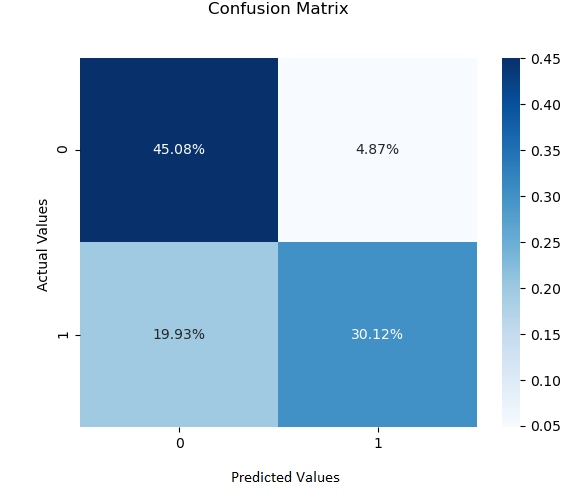
\includegraphics[width=\textwidth,height=\textheight,keepaspectratio]{images/image2.png}
    \caption{Matriu de confusió}
    \label{fig:matriuConfusio}
\end{figure}